\chapter{Results and discussion}
\section{Exemplary analysis of pump-probe trace}
The analysis of the pump-probe time traces was either done by fitting the data or by applying a fast fourier transform (FFT).
We can measure and analyze the rotation of polarization as the normalized difference between the two photodiode inputs and the transient reflectivity as the sum of the two photodiode inputs.
In \autoref{fig:example_analysis_fit}b we use a suitable dataset of rotation of polarization to demonstrate both of these methods.
\begin{figure}[ht]
    \centering
    \includegraphics{pictures/plots/example_analysis_fit.pdf}
    \caption{\textbf{a)} An example trace analyzed using the fitting functions \autoref{eqn:fit_hf} and \autoref{eqn:fit_lf}. \textbf{b)} After subtracting a linear background an FFT was applied, producing this plot.}
    \label{fig:example_analysis_fit}
\end{figure}
\FloatBarrier
The upper part of \autoref{fig:example_analysis_fit}a shows the data as well the first "lf-fit", indicated by a solid red line, done to extract the frequency $f_{\text{lf}}$ and amplitude $A_{\text{lf}}$ of the lower frequency mode by fitting
\begin{equation}
    f(t) = A_{\text{lf}} \cdot \exp(-\lambda_{\text{lf}} t) \cdot \cos(2 \pi f_{\text{lf}} t + \phi_{\text{lf}}) + C \cdot \exp(-\lambda t) + D \cdot x + E
    \label{eqn:fit_lf}
\end{equation}
to the data.
$\lambda_{\text{lf}}$ represents the decay constant of the lf-oscillation and $\phi_{\text{lf}}$ is its phase.
From the viewpoint of the higher frequency mode the lower frequency mode resembles more of a background which is why any exponential and linear contributions to the background are also included in \autoref{eqn:fit_lf}.
% In relation to the higher frequency mode the lower frequency mode resembles more of a background which is why any exponential and linear contributions to the background are also included in \autoref{eqn:fit_lf}.
After subtracting the GHz-fit from the data the simpler fit function
\begin{equation}
    f(t) = A_{\text{hf}} \cdot \exp(-\lambda_{\text{hf}} t) \cdot \cos(2 \pi f_{\text{hf}} t + \phi_{\text{hf}}) \;,
    \label{eqn:fit_hf}
\end{equation}
only featuring an exponentially decaying sine-wave, is used to extract the frequency $f_{\text{hf}}$ and amplitude $A_{\text{hf}}$ of the hf-mode.
This fit is depicted in the lower part of \autoref{fig:example_analysis_fit}a by the red line.
The results of both fits are shown in \autoref{fig:example_analysis_fit}b as the red markers.

Since the only important parameters in the context of this thesis are the amplitude and the frequency of the modes, the FFT represents another approach for the data analysis.
Here, only the background is fitted in preparation for applying the FFT, so that the oscillations are singled out and so that they can be broken down into a linear combination of sine or cosine functions, as is the premise of a fourier transform.
A discrete fourier transform of a perfectly sinusoidal signal yields an infinitely thin peak at one exact frequency.
The exponential decay of the oscillation in the time-domain translates to a finite width of the resulting peak in the frequency domain together with a reduction in the height of the peak.
This effect is called dephasing and happens because the amplitudes get redistributed over more frequency bins, as the uncertainty rises.
The faster the decay happens, the wider the peak gets, as you can see in \autoref{fig:example_analysis_fit} for both of the modes.
The peak of the FFT associated with the lf-mode is much lower than the amplitude acquired through the fit.
The peak of the hf-mode is also slightly lower than the amplitude of the fit which is also attributed to the same effect, albeit to a smaller extent.

But more importantly, if no decay is visible in the observed time interval, this effect can be neglected.
In view of this, the fitting method is used to analyze the measurements on NiO/C60, as a clear decay is visible there.
The FFT method is used for the measurements of NiPS3, since no decay of the oscillations is discernable.


\section{NiO/C60}
\subsection{Absorption measurements on NiO/C60}
As described in ....., NiO is as a prototypical antiferromagnet which was already a subject of much research effort.
In this thesis we focus on the changes we can detect in the magnetic behavior by covering the NiO with a molecular layer.
To try this, C60 was used in part because it is widely available, but mainly because of its strong interaction with ferromagnetic surfaces \lit{Veenstra}.
% C60 is a molecule which is
% (strong surface dipole formation) when in contact with () ..... 
Assuming that C60 changes the magnetic anisotropy which has a direct influence on the magnon frequency in NiO it is adsorbed on its surface.
\begin{figure}[ht]
    \centering
    \includegraphics[width=0.7\textwidth]{pictures/plots/NiO_absorption_nm.pdf}
    \caption{Absorption spectra measured on the CARY system for pure NiO (blue line) and for NiO/C60 (red line). The lower part is a zoom-in on the d-d transition.}
    \label{fig:NiO_absorption_nm}
\end{figure}
\FloatBarrier
Ahead of the time-resolved measurements, static absorption spectra were acquired using the commercial spectroscopy Cary 6000i system by Agilent.
Two \qty{15}{nm} thick NiO samples were measured, one pure NiO sample and one NiO sample with the adsorbed C60-molecules.
\autoref{fig:NiO_absorption_nm} shows the absorption spectra of both of the samples in the range of 1000 to \qty{1500}{nm}.
As the two samples did not have the same size, a direct comparison of the two spectra by subtraction or division was not possible.
Nonetheless, an obvious broadening of the exciton peak at \qty{1280}{nm} and the magnon-sideband at \qty{1273}{nm} is visible in the spectrum of NiO/C60 in \autoref{fig:NiO_absorption_nm}, especially in the zoomed-in view on the bottom.
While still being distinct, the exciton-magnon (X-M) peaks of NiO/C60 seem to have shifted slightly to higher energies by about \qty{1}{meV} with respect to the ones froms the pure NiO.
Furthermore, some additional features between \qty{1350}{nm} and \qty{1400}{nm} are clearly visible in the spectrum of the NiO/C60 in contrast to the one from the pure NiO and may be worthwhile to examine.

\subsection{Pump wavelength dependence of NiO/C60}
A pump wavelength dependence around the X-M peak (\qty{0.97}{eV}) on pure NiO has already been performed by Bossini et al. \lit{Bossini et al.} which is also featured here and which some of the following explanations are based on.
Now we want to see what impact the hybridization of the pure NiO surface with the C60 molecule layer has on the domain structure and thus on the coupling of the two magnon modes.

The pump wavelength dependence consists of measurements taken at different pump wavelenghts ranging from \qty{1158}{nm} to \qty{1362}{nm}, which are shown in \autoref{fig:NiO_pump_WL_dependence}.
The traces cover a time interval of around \qty{25}{ps} ensuring that they encompass at least three whole periods of the lf-mode each lasting \qty{7.7}{ns}.
The start of the cross-correlation was taken as the zero point in the plot.
To extract the frequency and amplitude of the lf-oscillations the data was fitted using the fit function \autoref{eqn:fit_lf}.
The fits are indicated by the red lines in the plot. 
Due to the absence of any lf-oscillations, it was not possible to fit the two uppermost traces and thus no red lines were plotted along them.
After subtracting the fits of the hf-mode from the initial data we get the plots featured in \autoref{fig:NiO_pump_WL_dependence_THz}.
Now only the hf-oscillations remain and thus an exponentially decaying sine-wave \autoref{eqn:fit_hf} is used to fit the data, which is again indicated by the red lines.
\begin{figure}[ht]
    \centering
    \includegraphics{pictures/plots/NiO_pump_WL_dependence.pdf}
    \caption{The time traces taken with pump-probe spectroscopy for different pump wavelengths ranging from \qty{1158}{nm} to \qty{1362}{nm} are shown here. As the two oscillations are well-pronounced in these plots, an analysis by fitting the data was chosen. The red line depicts the fit of the lf-mode together with the background.}
    \label{fig:NiO_pump_WL_dependence}
\end{figure}
\FloatBarrier
The two extracted frequencies from each dataset are then plotted against their respective energies in \autoref{fig:NiO_pump_WL_dependence_freq}.
For the hf-mode the plot resembles a straight line with a constant frequency at \qty{1.07}{THz}.
This coincides with the values found in several literature sources \lit{3 magnon modes}.
The values for the lf-mode also stay about the same throughout the different pump energies, varying between 0.12 and \qty{0.15}{THz} with an average of \qty{0.13}{THz}.
% They shift slightly more than the hf-frequency.
% However, the uncertainty intervals given by the fits overlap heavily, so that an average frequency at around \qty{0.13}{THz} can be established, which is again corroborated by literature \lit{magnon modes}.
\begin{figure}[ht]
    \centering
    \includegraphics{pictures/plots/NiO_pump_WL_dependence_THz.pdf}
    \caption{The measured data is shown after subtracting the fit of the lf-mode from it. The red line shows the fit of the hf-mode. The two uppermost traces are not featured, as they could not be fitted and thus the hf-mode could not be singled out.}
    \label{fig:NiO_pump_WL_dependence_THz}
\end{figure}
\FloatBarrier
In contrast to the WL dependence of the frequency the change in amplitude for different pump wavelengths is much more obvious and can already clearly be seen in \autoref{fig:NiO_pump_WL_dependence}.
Following the same procedure as for the frequencies, in \autoref{fig:NiO_pump_WL_dependence_ampl} the spectral dependence of the amplitudes of the two magnon modes is displayed in dark orange and dark blue.
\begin{figure}[ht]
    \centering
    \includegraphics{pictures/plots/NiO_pump_WL_dependence_freq.pdf}
    \caption{Here, the pump wavelength dependencies of the frequency of both the LF- and the HF-modes in NiO/C60 are shown.}
    \label{fig:NiO_pump_WL_dependence_freq}
\end{figure}
\begin{figure}[ht]
    \centering
    \includegraphics{pictures/plots/NiO_pump_WL_dependence_ampl.pdf}
    \caption{Here, the pump wavelength dependencies of the amplitudes of both the LF- and the HF-modes in NiO/C60 are shown. Underlayed in paler colors, is the data for pure NiO. To make a comparison possible, every dependence is normalized to its highest value.}
    \label{fig:NiO_pump_WL_dependence_ampl}
\end{figure}
\FloatBarrier
Comparing it to the absorption spectra a clear broadening of the resonance can be seen, as the ultrashort laser pulses have a pulse duration of \qty{75}{fs} and thus a finite bandwidth of about \qty{40}{meV}.
Under the assumption that the spectral shape of the laser pulses is gaussian the position maxima of the spectral dependencies should not change.
Here, a comparison between the data taken on the \qty{15}{nm} thick NiO crystal with and without adsorbed C60 molecules is done.
The pale colored curves in the background show the data on pure NiO and the ones in deeper colors show the measurements done on the NiO/C60 system.
It should be noted here, that the measurements on the pure NiO were done previously within the scope of preliminary measurements.
On the basis of the absorption spectrum as seen in \autoref{fig:7}, different areas can be identified in the spectral dependencies.
The range of non-resonant pumping before exciting the X-M peak up to about \qty{0.95}{eV} shows nearly no amplitude for both magnon modes.
Albeit, in contrast to the hf-mode the lf-mode demonstrates a slightly higher value which is explained in terms of Impulsive Stimulated Raman Scattering (ISRS) \lit{C. Tzschaschel} meaning that slightly off-resonant excitation is also possible.
ISRS is thought of as an effective magnetic field exerting maximum torque on spins lying perpendicular to it, so that the contributions from different T-domains do not cancel out eachother \lit{2 Kirilyuk}.
Next, the energy range 0.95-\qty{0.99}{eV} is described.
Representing the area where the pump energy covers the X-M peak at around \qty{0.97}{eV}, with a tolerance of half of the pulse bandwidth, it features a prominent amplification of both modes.
The coherent amplification of the hf-mode is easy to understand as the pump induces the X-M transition previously explained in \autoref{sec:x_m}.
\begin{figure}[ht]
    \centering
    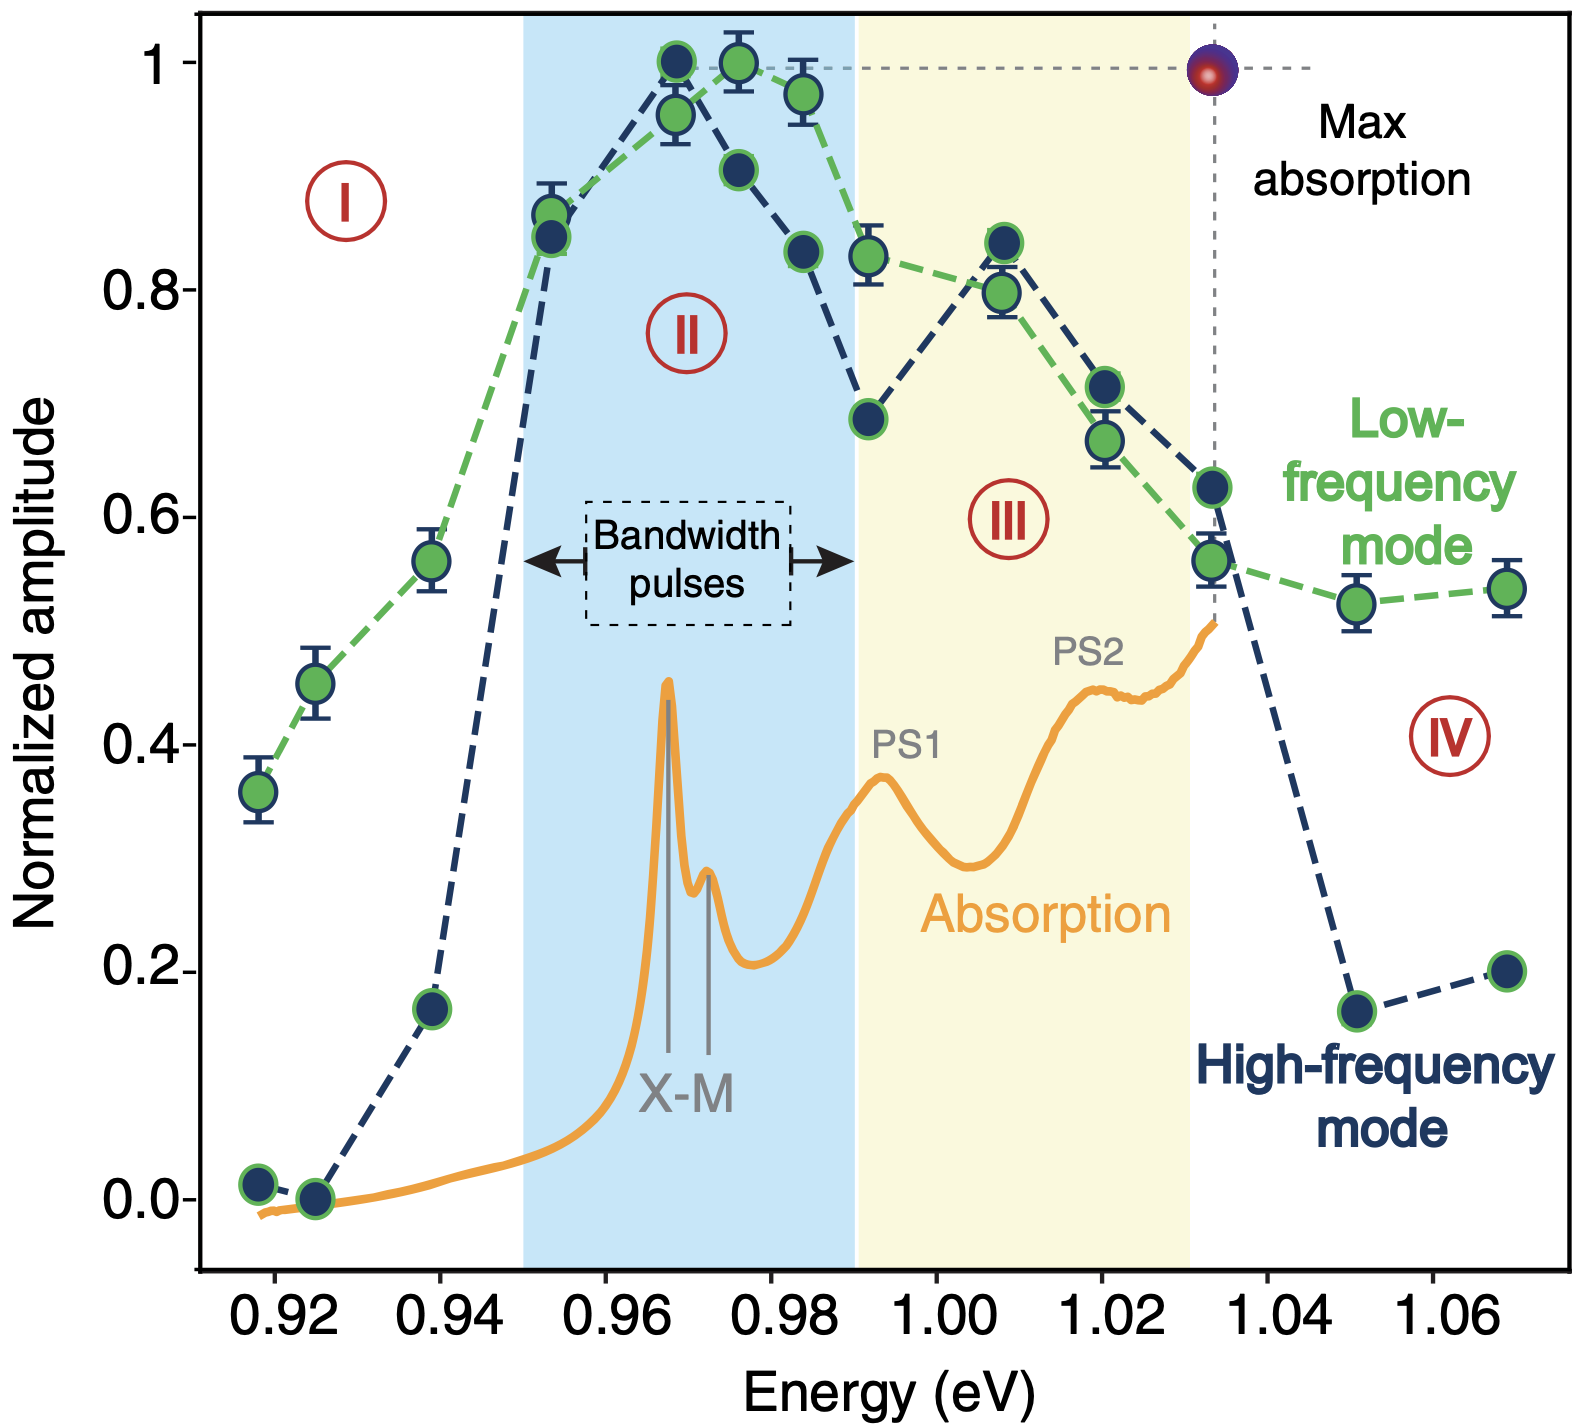
\includegraphics[width=0.5\textwidth]{pictures/7.png}
    \caption{The spectral dependence of the magnon modes in a \qty{100}{micrometer} thick NiO crystal measured in transmission. The dependecies are normalized to their highest values. Taken from \lit{Bossini et al.}}
    \label{fig:7}
\end{figure}
\FloatBarrier
What is surprising here, is the simultaneous amplification of the lf-mode in the same region, although it does not participate in the X-M transition.
The source of this behaviour is the multidomain state of the NiO sample yielding a coupling between the two modes mediated by the oscillating domain wall motion as explained in \autoref{sec:mode_coupling}.
The third region of the spectral dependencies exhibits a smaller peak at about \qty{1.03}{eV}.
This is due to the presence of phonon sidebands PS1 and PS2 belonging to the exciton peak which, when pumped, induces the X-M transition \lit{Bossini}.
The phonon sidebands also represent a new absorption channel for the pump light, the consequences of that being a smaller amplification as some of the pump power is absorbed by the lattice.
Finally, in the fourth region the amplitude of both modes sinks down to a negligible value again.

The amplitudes of the modes on the NiO/C60 sample follow roughly the same trend.
The most apparent difference appears to be a slight shift of the amplification peak of 10-\qty{20}{meV} to higher energies.
Seemingly, the molecule coverage also narrows down the amplification resulting in a more distinct peak.
Furthermore, the height of the phonon sideband induced amplification around \qty{1.03}{eV} relative to the resonant amplification at the X-M peak is reduced.
This reinforces the impression of it being sharper as well.
% Furthermore, a reduction of the height of the phonon sideband induced amplification relative to the resonant amplification at the X-M peak can be observed which would reinforce the impression of it being sharper as well.

\begin{figure}[ht]
    \centering
    \includegraphics{pictures/plots/NiO_pump_1278nm_comparison.pdf}
    \caption{A comparison between the two measurements at \qty{1278}{nm} pump before measuring the absorption and after, to show the decrease in signal quality.}
    \label{fig:NiO_pump_1278nm_comparison}
\end{figure}
In order to get more points around the amplification peak, another set of measurements was done after the absorption measurements in this second region.
Now, a stepsize of \qty{0.1}{eV} in the energy range of 0.95 to \qty{1.02}{eV} was choosen for the pump, doubling the resolution of the spectral dependence.
A tremendeous decrease in signal quality, compared to the measurements before, can be seen.
The hf-oscillation are still easily discernible, but a noticeable reduction of their quality took place.
The lf-mode on the other hand became nearly indistinguishable.
For a direct comparison the measured traces at \qty{1278}{nm} (\qty{0.97}{eV}) pump were plotted next to eachother in \autoref{fig:NiO_pump_1278nm_comparison}.
It is assumed that during the process of taking the absorption measurements some kind of contaminant adsorbed on the surface or the surface got scratched.
This would make the surface uneven, which in turn weakens the coherence of the modes leading to a compromised signal.
\begin{figure}[ht]
    \centering
    \includegraphics{pictures/plots/NiO_pump_WL_dependence_2.pdf}
    \caption{The time traces for different pump wavelengths ranging from \qty{1215}{nm} to \qty{1305}{nm} are shown here. The same procedure as in \autoref{fig:NiO_pump_WL_dependence} was also applied here.}
    \label{fig:NiO_pump_WL_dependence_2}
\end{figure}

The same procedure as before was applied to analyze the data in \autoref{fig:NiO_pump_WL_dependence_2}.
As is clearly visible, the amplitude of the lf-mode is reduced to a vanishing value.
This means that the reliability of the fits of the lf-mode is diminished, as a slight variation of the less important fit parameters results in a substantial change in the two most significant fit parameters, the amplitude and to a lesser extent, the frequency.
The hf-mode on the other hand, except the \qty{1305}{nm}-pump trace, allows for a precise fit and a more reliable interpretation.
The amplification peak still looks sharper than in the NiO sample showing a clear change caused by the adsorbed C60 molecules.
\begin{figure}[ht]
    \centering
    \includegraphics{pictures/plots/NiO_pump_WL_dependence_ampl_2.pdf}
    \caption{Here the spectral dependencies of the amplitudes of both the LF- and the HF-modes in NiO/C60 are shown with an improved energy resolution. Every dependence is normalized to its highest value.}
    \label{fig:NiO_pump_WL_dependence_ampl_2}
\end{figure}
\FloatBarrier

\subsection{Measurements at 1400nm pump WL}
Another noticeable feature in the absorption spectrum in \autoref{fig:NiO_absorption_nm} are small peaks around \qty{1400}{nm}.
Pumping at this wavelength resulted in the green trace shown in \autoref{fig:NiO_pump_1400nm_1320nm}.
For the sake of reference, the pump was also set to \qty{1320}{nm} as in that area of the absorption spectrum no features can be discerned which represents the absence of any possible dynamics.
The data taken with \qty{1400}{nm} pump displays a feature in the first few picoseconds which persists at different pump powers and temperatures and does not change its shape.
This is taken as a reason to exclude this part of the trace from the analysis.
For the analysis an exponential background was subtracted depicted by the red line.
The subsequent FFT is shown in \autoref{fig:NiO_pump_1400nm_1320nm_FFT}.
\begin{figure}[ht]
    \centering
    \includegraphics{pictures/plots/NiO_pump_1400nm_1320nm.pdf} \vspace{-0.3cm}
    \caption{The time evolution after pumping in a region without any features at \qty{1320}{nm} and the one after pumping at \qty{1400}{nm}, where some features in the absorption spectrum of NiO/C60 can be seen in \autoref{fig:NiO_absorption_nm}.}
    \label{fig:NiO_pump_1400nm_1320nm}
\end{figure}
% \FloatBarrier
\begin{figure}[ht]
    \centering
    \includegraphics{pictures/plots/NiO_pump_1400nm_1320nm_FFT.pdf} \vspace{-0.3cm}
    \caption{The FFT of both traces at \qty{1320}{nm} and \qty{1400}{nm} pump.}
    \label{fig:NiO_pump_1400nm_1320nm_FFT}
\end{figure}
\FloatBarrier
The FFT of the \qty{1320}{nm}-data shows no distinct peaks.
This supports the assumption of the lack of any induced dynamics at this pump wavelength.
Contrary, the \qty{1400}{nm}-data exhibits a clear peak at \qty{0.62}{THz} standing out from the background noise, although it is very low in amplitude.
A mode with this frequency is not yet reported in literature and it is not completely evident if and what physical meaning it has.
(For the purpose of clarifying this question a temperature dependence was carried out... hier weiß ich nicht, ob ich das überhaupt zeigen sollte, weil es wirklich gaarnichts aussagt)

\section{NiPS3}
Another interesting compound containing Ni is NiPS3, which belongs to the group of van-der-Waals antiferromagnets.
Just like in NiO, the magnetism stems from the Ni$^{2+}$-ions.
It also exhibits a d-d transition centered at \qty{1.1}{eV} originating from the Ni$^{2+}$-ions \lit{Belvin}.
A paper from Afanasiev et al. \lit{Afanasiev} exists that deals with the magnon dynamics in NiPS3.
It mainly describes the selective activation of a magnon mode by resonantly pumping the d-d transition with light.
Furthermore, the pump polarization dependence of the magnon mode is investigated.
% It shows that it arises from the light-induced magnetic anisotropy resulting from the excitation of the higher-energy states of Ni-ions.
\autoref{fig:9} depicts the amplitude of the observed magnon mode (pink) as a function of pump photon energy.
The relatively narrow resonance around the $^3A_{2\text{g}} \rightarrow ^3T_{2\text{g}}$ transition together with the dependence of the amplitude on the pump polarization angle reveals the qualitative origin of the in-plane mode.
The transition from the $^3A_{2\text{g}}$ ground state to the higher-energy $^3T_{2\text{g}}$ state induces a magnetic anisotropy which generates a suitably short torque impulsively triggering the magnon mode.
\begin{figure}[ht]
    \centering
    \begin{subfigure}[b]{0.5\textwidth}
        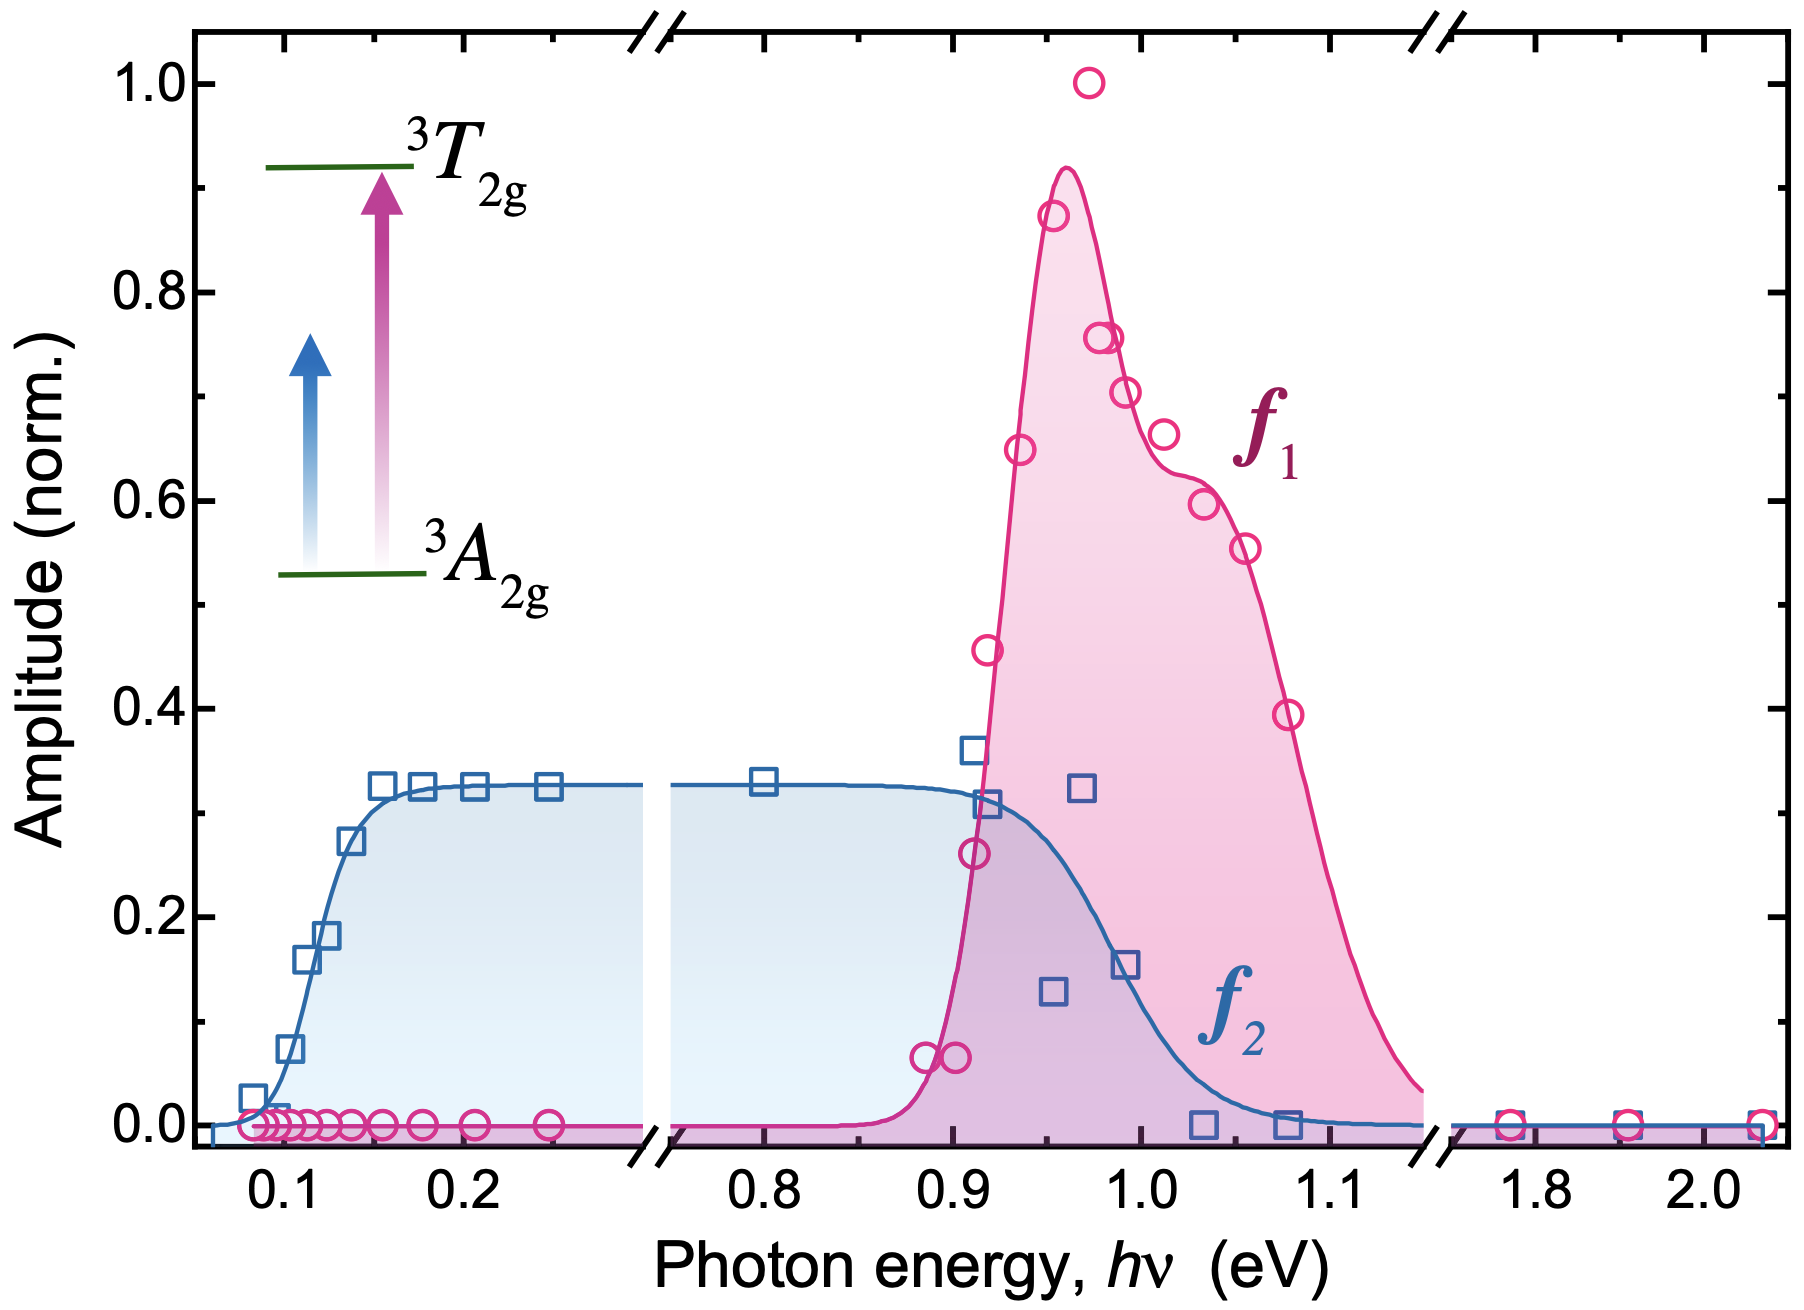
\includegraphics[width=\textwidth]{pictures/9.png}
        \caption{}
        \label{fig:9}
    \end{subfigure}
    \hspace{0.3cm}
    \begin{subfigure}[b]{0.28\textwidth}
        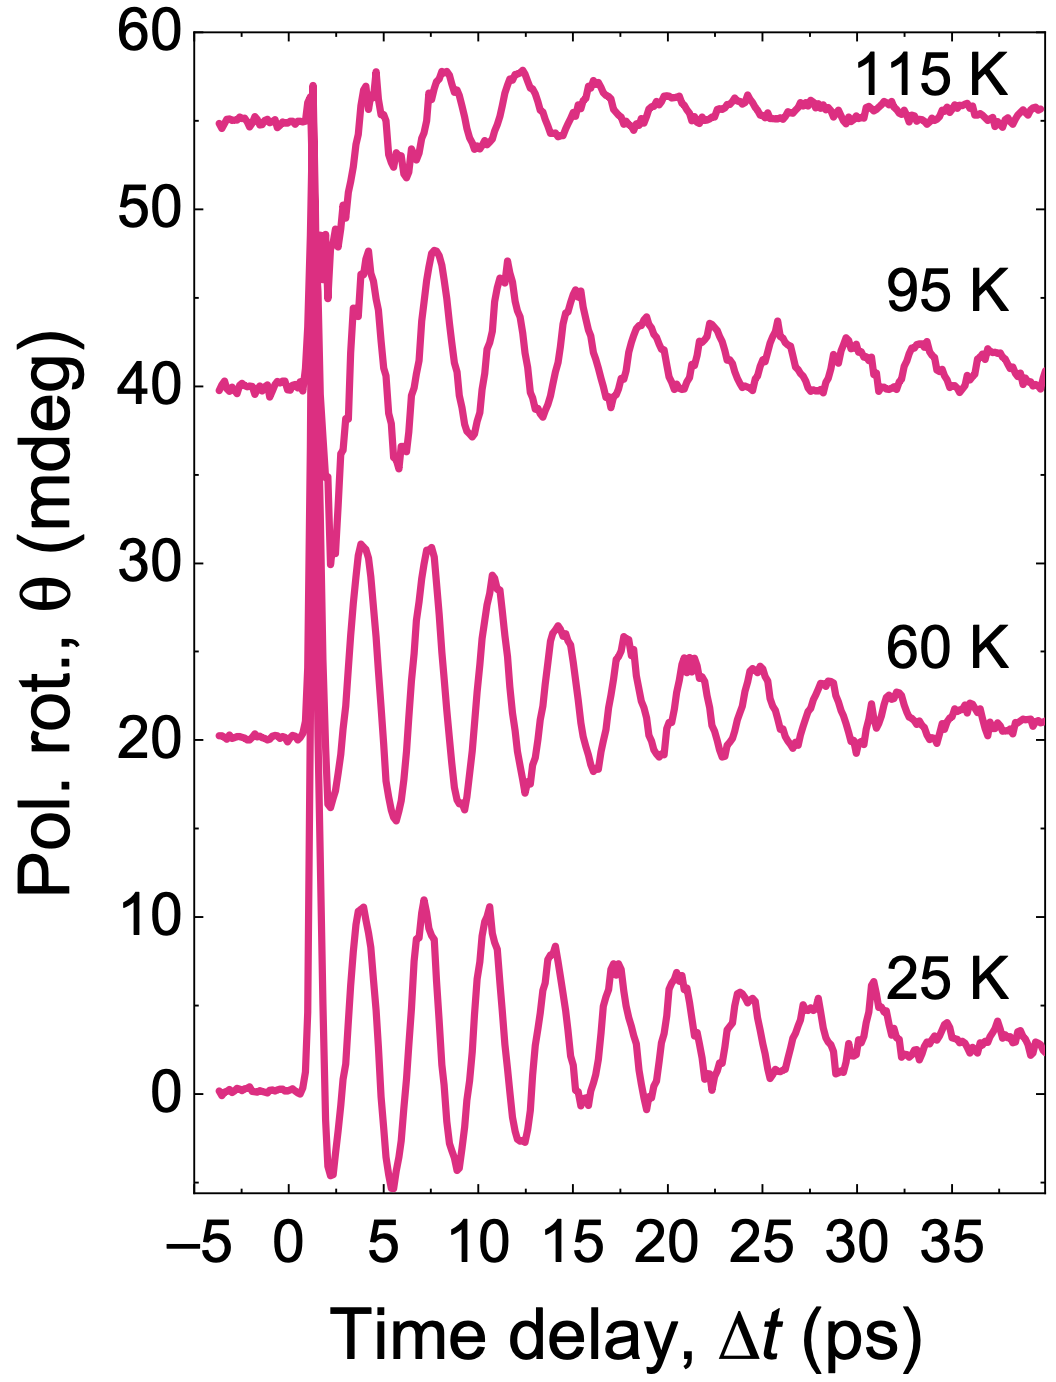
\includegraphics[width=\textwidth]{pictures/10.png}
        \caption{}
        \label{fig:10}
    \end{subfigure}
    \caption{\textbf{a)} The spectral dependencies of the amplitudes of the in-plane $f_1$ mode and the out-of-plane $f_2$ mode normalized to the maximum value of the $f_1$ mode. The solid lines are guides to the eye. \textbf{b)} The time-resolved rotation of polarization after pumping with an energy of \qty{1.08}{eV} at different temperatures. Both taken from \lit{Afanasiev et al.}}
\end{figure}
\FloatBarrier
First, an effort was undertaken to reproduce one of the already established results from that paper.
Namely, to detect the in-plane magnon mode with a frequency of \qty{0.3}{THz} while pumping at \qty{1.08}{eV} and probing at \qty{800}{nm} which is shown for different temperatures in \autoref{fig:10}.
\begin{figure}[ht]
    \centering
    \includegraphics{pictures/plots/NiPS3_no_magnons.pdf} \vspace{-0.3cm}
    \caption{The measurement taken on the NiPS3 flake at a \qty{1.09}{eV} or \qty{1136}{nm} pump show no oscillations in the rotation of polarization or the transient reflectivity after \qty{23}{ps} after the zero-delay.}
    \label{fig:NiPS3_no_magnons}
\end{figure}
\FloatBarrier
\autoref{fig:NiPS3_no_magnons} shows a time trace of the rotation of polarization until \qty{23}{ps} after a \qty{1.09}{eV} pump.
There are no oscillations visible.
The measurements were done at different polarization directions for the pump and the probe pulse and at varying fluences, but still no fluctuations appeared.
In contrast to \lit{Afanasiev, Toyoda} the measurements were not taken in transmission but in reflection.
Subsequent measurements using a magnetic field of up to \qty{2}{T}, to cant the spins more into the direction of the c-axis for an easier detection, show slight oscillations which only start after about \qty{30}{ps}.
It is possible, that the in-plane mode is first masked by the thermal demagnetization and then by the dominant GHz-modes decribed in the following.

Observing a longer timescale of around \qty{300}{ps} with the probe set to \qty{800}{nm} reveals two GHz-modes with the frequencies 13 and \qty{28}{GHz} which are labeled low-frequency (LFM) and high-frequency (LFM) mode, analogous to the two modes in NiO.
These modes are not yet described in literature.
Instead of fitting the oscillations, the easier method of FFT was used as the phase does not seem to change in the evaluated dependencies and only the amplitude and frequency are of importance to us.
It should be noted that the frequencies do not change from their values during the three measured dependencies and are therefore omitted from the following sections.

\subsection{Pump polarization dependence}
To help us understand the excitation mechanism behind the GHz-modes a pump polarization dependence is carried out.
For this purpose the rotation of polarization and the transient reflectivity was analyzed while changing the angle from 0° to 180° with a stepsize of 15°.
The probe polarization angle was set to 150° for the duration of this dependence.
Employing an FFT the amplitude along with the frequency of the detected oscillation are extracted.
A beating of two different oscillations is clearly visible in \autoref{fig:NiPS3_pump_polarization_dependence_diff}.
\begin{figure}[hbt!]
    \centering
    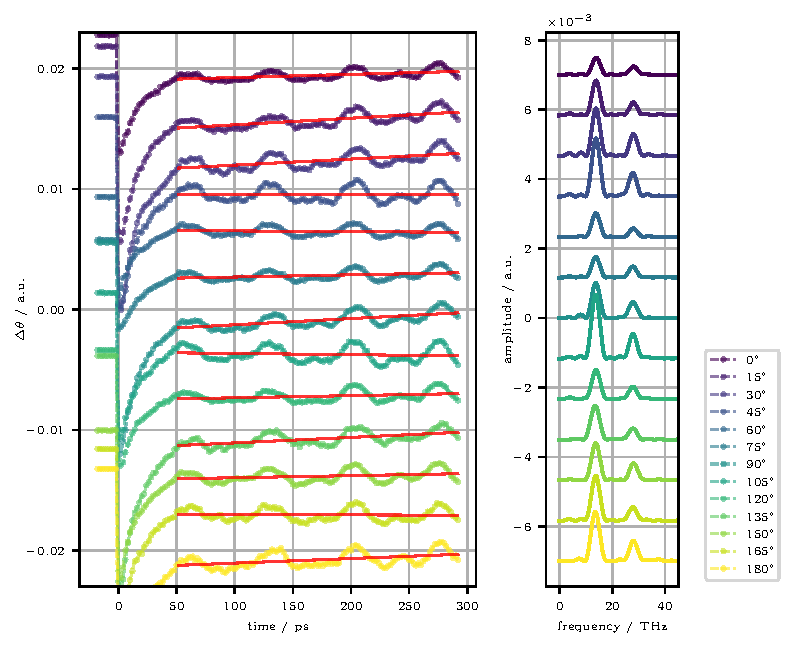
\includegraphics{pictures/plots/NiPS3_pump_polarization_dependence_diff.pdf} \vspace{-0.3cm}
    \caption{\textbf{a)} Rotation of polarization as a function of time taken at pump polarization angles ranging from 0° to 180° with a stepsize of 15°. The red lines depict the linear background. \textbf{b)} The FFTs of the traces at the different pump polarization angles display two prominent modes at \qty{13}{GHz} (LFM) and \qty{28}{GHz} (HFM).}
    \label{fig:NiPS3_pump_polarization_dependence_diff}
\end{figure}
\FloatBarrier
\begin{figure}[hbt!]
    \centering  
    \includegraphics{pictures/plots/NiPS3_pump_polarization_dependence_diff_ampl.pdf} \vspace{-0.3cm}
    \caption{The extracted amplitudes of the lf- and hf-mode in the rotation of polarization plotted against the pump polarization angle and normalized to the maximum value. The data traces were taken at a probe polarization of 150°. The continuous lines show the sinusoidal fit which yields a 3-fold symmetry.}
    \label{fig:NiPS3_pump_polarization_dependence_diff_ampl}
\end{figure}
\FloatBarrier
Considering the dependence in \autoref{fig:NiPS3_pump_polarization_dependence_diff_ampl}, a clear sinusoidal shape with a period of 60° be seen.
It is hard to determine to what crystallographic directions the angles of the orientation of polarization correspond to, as no literature on these modes is available yet, their origin is ambiguous and no dependencies of known features were done to identify the orientation of the sample in relation to our setup.
Nonetheless, the 3-fold symmetry of both modes is recognizable which indicates their origin to be associated with the 2D-lattice of the Ni$^{2+}$-ions as the honeycomb structure has the same symmetry.

The transient reflectivity in \autoref{fig:NiPS3_pump_polarization_dependence_sum} shows only one distinct mode, the hf-mode, as do all following transient reflectivity measurements.
As the transient reflectivity is regarded as a measure for non-magnetic dynamics this indicates that the hf-mode emerges from lattice dynamics.
The amplitude of the hf-mode in the transient reflectivity in \autoref{fig:NiPS3_pump_polarization_dependence_sum_ampl} also displays a 3-fold symmetry in regard to the pump polarization.
Furthermore, the same periodicities in the pump polarization dependencies for the rotation of polarization and transient reflectivity suggest that both the modes have a common origin.
Both polarization dependencies show some data points deviating from the sinusoidal shape in the region of 140°, implying some issues arising from the setup.
A possible explanation could be that the $\frac{\lambda}{2}$-plate used to adjust the polarization angle has a faulty spot.
As the pump does not hit the waveplate exactly in the middle, a change of angle would change the spot where the pump meets plate.
Aside from that, the other points fit into the shape quite well.
\begin{figure}[hbt!]
    \centering
    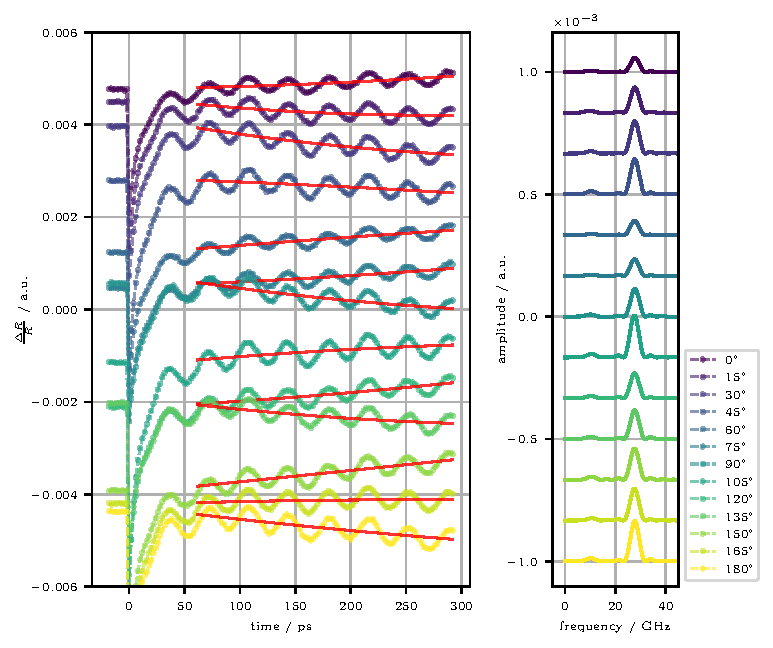
\includegraphics{pictures/plots/NiPS3_pump_polarization_dependence_sum.pdf} \vspace{-0.3cm}
    \caption{\textbf{a)} Transient reflectivity as a function of time taken at pump polarization angles ranging from 0° to 180° with a stepsize of 15°. The red lines depict the linear background. \textbf{b)} The FFTs of the traces at the different pump polarization angles display one prominent mode at \qty{28}{GHz}.}
    \label{fig:NiPS3_pump_polarization_dependence_sum}
\end{figure}
% \FloatBarrier
\begin{figure}[hbt!]
    \centering  
    \includegraphics{pictures/plots/NiPS3_pump_polarization_dependence_sum_ampl.pdf} \vspace{-0.3cm}
    \caption{The extracted amplitudes of the hf-mode in the transient reflectivity plotted against the pump polarization angle and normalized to the maximum value. The data traces were taken at a probe polarization of 150°. The continuous line shows the sinusoidal fit which yields a 3-fold symmetry.}
    \label{fig:NiPS3_pump_polarization_dependence_sum_ampl}
\end{figure}
\FloatBarrier

\newpage
\subsection{Probe polarization dependence}
The probe polarization dependence analyzed in this chapter makes a statement about the detection mechanism behind the oscillations we observe in the rotation of polarization seen in \autoref{fig:NiPS3_probe_polarization_dependence_diff}a.
For the following measurements the pump polarization angle was set to 180° and the probe polarization angle was varied from 0° to 180° with a stepsize of 15°.
As for the detection mechanism two magneto-optical effects come into question:
The magneto-optical Kerr effect (MOKE) which originates from a possible out-of-plane magnetization component and the Cotton-Mouton effect originating from an in-plane component of the Neél vector causing linear birefringence.
The Faraday effect does not depend on the polarization angle of the probe \lit{Toyoda}.
Using the same procedure as for the pump polarization dependence, the amplitudes of the oscillations in \autoref{fig:NiPS3_probe_polarization_dependence_diff} are extracted via FFT.
\autoref{fig:NiPS3_probe_polarization_dependence_diff_ampl} portrays the amplitudes of both the lf- and hf-mode as a function of the probe polarization angle.
The continous lines display sinusoidal fits.
Taking the angle dependence in \autoref{fig:NiPS3_probe_polarization_dependence_diff_ampl} into account, the conclusion can be drawn that the observed signal stems from linear birefringence, as theory also suggests that such a 2-fold symmetry corresponds to linear birefringence \lit{Satoh}.
It is also visible that the amplitude completely vanishes at the minima of the sinusoidal curve.
\begin{figure}[hbt!]
    \centering
    \includegraphics{pictures/plots/NiPS3_probe_polarization_dependence_diff.pdf} \vspace{-0.3cm}
    \caption{\textbf{a)} Rotation of polarization as a function of time taken at probe polarization angles ranging from 0° to 180° with a stepsize of 15°. The red lines depict the linear background. \textbf{b)} The FFTs of the traces at the different probe polarization angles display two prominent modes at \qty{13}{GHz} and \qty{28}{GHz}.}
    \label{fig:NiPS3_probe_polarization_dependence_diff}
\end{figure}
% \FloatBarrier
\begin{figure}[hbt!]
    \centering  
    \includegraphics{pictures/plots/NiPS3_probe_polarization_dependence_diff_ampl.pdf} \vspace{-0.3cm}
    \caption{The extracted amplitudes of the lf- and hf-mode in the rotation of polarization plotted against the probe polarization angle and normalized to the maximum value. The data traces were taken at a pump polarization of 180°. The continuous lines show the sinusoidal fit which yields a 2-fold symmetry.}
    \label{fig:NiPS3_probe_polarization_dependence_diff_ampl}
\end{figure}
\FloatBarrier
\autoref{fig:NiPS3_probe_polarization_dependence_diff} shows the measured transient reflectivity for the different probe polarization angles together with the respective FFT which again only yields the hf-mode.
The probe polarization dependence of the transient reflectivity plotted in \autoref{fig:NiPS3_probe_polarization_dependence_sum_ampl} displays the same periodicity as the rotation of polarization.
\begin{figure}[hbt!]
    \centering
    \includegraphics{pictures/plots/NiPS3_probe_polarization_dependence_sum.pdf} \vspace{-0.3cm}
    \caption{\textbf{a)} Transient reflectivity as a function of time taken at probe polarization angles ranging from 0° to 180° with a stepsize of 15°. The red lines depict the quadratic background. \textbf{b)} The FFTs of the traces at the different probe polarization angles display one prominent mode at \qty{28}{GHz}.}
    \label{fig:NiPS3_probe_polarization_dependence_sum}
\end{figure}
% \FloatBarrier
\begin{figure}[hbt!]
    \centering  
    \includegraphics{pictures/plots/NiPS3_probe_polarization_dependence_sum_ampl.pdf} \vspace{-0.3cm}
    \caption{The extracted amplitudes of the hf-mode in the transient reflectivity plotted against the probe polarization angle and normalized to the maximum value. The data traces were taken at a pump polarization of 180°. The continuous line shows the sinusoidal fit which yields a 2-fold symmetry.}
    \label{fig:NiPS3_probe_polarization_dependence_sum_ampl}
\end{figure}
\FloatBarrier

\subsection{Temperature dependence}
The temperature dependence was measured to be able to determine whether the two modes are of magnetic or non-magnetic origin.
The pump and probe polarizations were set to 180° and 150°, as this combination of angles yielded the smoothest oscillations.
The temperature was varied from 77 to \qty{170}{K} with a stepsize of \qty{10}{K} except around the Neél temperature (\qty{155}{K}), where the stepsize was reduced to \qty{5}{K}.
What we see now in \autoref{fig:NiPS3_temp_dependence_diff} is that both modes completely vanish above a certain temperature.
For the lf-mode this temperature coincides with the Neél temperature, which proves a connection to the magnetic system.
For the hf-mode whose detected amplitude is always smaller than the one from the lf-mode, any noticeable amplitude value vanishes after around \qty{120}{K}.
\begin{figure}[hbt!]
    \centering
    \includegraphics{pictures/plots/NiPS3_temp_dependence_diff.pdf} \vspace{-0.3cm}
    \caption{\textbf{a)} Rotation of polarization as a function of time acquired at temperatures ranging from 77 to \qty{170}{K} with an approximate stepsize of \qty{10}{K}. The blue lines depict the linear background. \textbf{b)} The FFTs of the traces at the different temperatures display two prominent modes at \qty{13}{GHz} and \qty{28}{GHz} which both vanish at two distinct temperatures.}
    \label{fig:NiPS3_temp_dependence_diff}
\end{figure}
% \FloatBarrier
\begin{figure}[hbt!]
    \centering  
    \includegraphics{pictures/plots/NiPS3_temp_dependence_diff_ampl.pdf} \vspace{-0.3cm}
    \caption{The exctracted amplitudes of the lf-mode in the rotation of polarization plotted against the temperatures, the respective data traces were taken at. A vanishing of the amplitudes after the Neél temperature is observed.}
    \label{fig:NiPS3_temp_dependence_diff_ampl}
\end{figure}
\FloatBarrier
As the transient reflectivity reflects the lattice dynamics, the amplitudes are not expected to be temperature dependent.
This is supported by the amplitude values of the hf-mode in \autoref{fig:NiPS3_temp_dependence_sum_ampl} being random, not following any trend and persisting even after the Neél temperature.
It can be concluded that the hf-mode originates in the lattice.
It couples to the magnetic system and induces dynamics which scale with the magnetic order.
\begin{figure}[hbt!]
    \centering
    \includegraphics{pictures/plots/NiPS3_temp_dependence_sum.pdf} \vspace{-0.3cm}
    \caption{\textbf{a)} Transient reflectivity as a function of time acquired at temperatures ranging from 77 to \qty{170}{K} with an approximate stepsize of \qty{10}{K}. The blue lines depict the linear background. \textbf{b)} The FFTs of the traces at the different temperatures display one prominent mode at \qty{28}{GHz}.}
    \label{fig:NiPS3_temp_dependence_sum}
\end{figure}
% \FloatBarrier
\begin{figure}[hbt!]
    \centering  
    \includegraphics{pictures/plots/NiPS3_temp_dependence_sum_ampl.pdf} \vspace{-0.3cm}
    \caption{The exctracted amplitudes of the hf-mode in the transient reflectivity plotted against the temperatures, the respective data traces were taken at. There is no clear trend visible.}
    \label{fig:NiPS3_temp_dependence_sum_ampl}
\end{figure}
\FloatBarrier


